% ---
% Reemplaza líneas 2771–2841 de Docs/Technical_Report.tex.
% Decisiones que lo respaldan: D-013, D-014, D-015, D-016, D-017, D-027, D-030,
% D-031, D-035, H-012, H-019, H-031, H-034, H-053.
% ---

\subsection{Módulo 5: Transformación}
\label{sec:modulo5}

El módulo de transformación implementa las cinco condiciones experimentales del estudio. Todas
parten del mismo vector $\mathbf{x} \in [0,\pi]^{12}$ producido por M4 y su salida alimenta en
paralelo dos módulos independientes: el análisis de separabilidad (M6) y la clasificación (M7).
La Tabla~\ref{tab:condiciones} resume las cinco condiciones.

\begin{table}[H]
\centering
\caption{Cinco condiciones experimentales del Módulo 5}
\label{tab:condiciones}
\renewcommand{\arraystretch}{1.3}
\begin{tabularx}{\textwidth}{@{}llXl@{}}
\toprule
\textbf{ID} & \textbf{Nombre} &
\textbf{Transformación} & \textbf{Tipo} \\
\midrule
C1 & Sin transformación & El vector $\mathbf{x}$ pasa directamente al clasificador. & Clásico \\
C2 & PCA lineal & Proyección sobre las 12 componentes principales. Es una rotación,
     así que actúa como control nulo. & Clásico \\
C3 & Kernel PCA (RBF) & Proyección no lineal a 12 dimensiones con núcleo gaussiano;
     $\gamma$ por la heurística de la mediana. & Clásico \\
C4 & \texttt{zz\_feature\_map} & Primer orden en $Z$ y acoplamiento $ZZ$, seguidos de
     \texttt{real\_amplitudes} con $\boldsymbol\theta$ fijo. Salida:
     $\langle Z_i\rangle\in[-1,1]^{12}$. & Cuántico \\
C5 & \texttt{pauli\_feature\_map}$(Y, ZZ)$ & Primer orden en $Y$ y el mismo acoplamiento $ZZ$,
     con el mismo \textit{ansatz} y $\boldsymbol\theta$. Salida:
     $\langle Z_i\rangle\in[-1,1]^{12}$. & Cuántico \\
\bottomrule
\end{tabularx}
\end{table}

\textbf{Sobre la condición C2.} Dado que M4 entrega un vector ya de dimensión $k=12$, una
proyección PCA a 12 componentes no constituye una reducción de dimensionalidad sino una
rotación ortogonal, que preserva las distancias euclidianas. En consecuencia, los índices
de Davies-Bouldin y Fisher y el \textit{kernel-target alignment} son invariantes ante ella,
y el perceptrón absorbe la rotación en su primera capa lineal. C2 se conserva
deliberadamente como \textbf{control nulo}: si las métricas de separabilidad arrojaran
valores distintos para C1 y C2, ello indicaría un defecto en su implementación. El
comparador clásico sustantivo es C3.

\textbf{Sobre la elección de C5.} La biblioteca Qiskit define \texttt{ZZFeatureMap} como un
caso particular de \texttt{PauliFeatureMap} con operadores $(Z, ZZ)$; ambas construcciones
preparan el mismo estado, con fidelidad $|\langle\phi_{ZZ}|\phi_{\text{Pauli}}\rangle|^2 = 1$.
Especificadas así, C4 y C5 no constituirían condiciones independientes. Se consideró
primero el conjunto $(X, ZZ)$, pero con una repetición el término en $X$ actúa sobre el
estado $|+\rangle$ que deja la capa de Hadamard, que es autoestado de $X$, y solo añade
una fase global: C5 equivaldría a un \textit{feature map} con únicamente el acoplamiento
$ZZ$. Se adopta por tanto el conjunto $(Y, ZZ)$. Sobre la esfera de Bloch, el giro en
$Z$ de C4 desplaza cada qubit a lo largo del ecuador y solo cambia una fase relativa,
mientras que el giro en $Y$ de C5 lo saca del ecuador y cambia las probabilidades de medir
0 y 1. Ambas condiciones comparten el acoplamiento $ZZ$ y el número de compuertas de
entrelazamiento, de modo que la comparación entre C4 y C5 mide el efecto del eje de la
codificación de primer orden.

Los parámetros $\boldsymbol\theta$ del \textit{ansatz} \texttt{real\_amplitudes}, 24 en total con
una repetición, se fijan una sola vez con una semilla declarada (42), muestreados de manera
uniforme en $[0,2\pi)$, y no se entrenan. Los valores esperados $\langle Z_i\rangle$ se calculan de
forma exacta a partir del vector de estado, una sola vez para todo el conjunto, y se guardan en
disco. El \textit{ansatz} no puede suprimirse. En C4, el \textit{feature map} aplica compuertas de Hadamard
seguidas de compuertas diagonales, que cambian las fases de las amplitudes pero no sus magnitudes.
Partiendo de $H^{\otimes k}|0\rangle$, toda amplitud conserva la magnitud $2^{-k/2}$, de modo que
$P(q_i = 0) = 1/2$ y $\langle Z_i\rangle = 0$ para cualquier entrada. La información codificada
reside en las fases, a las que una medición en la base $Z$ es insensible, y el \textit{ansatz} es lo
que las convierte en probabilidades medibles. En C5 el giro en $Y$ sí cambia las probabilidades, pero
sin el \textit{ansatz} $\langle Z_i\rangle = -\sin(2x_i)$ dependería de una sola característica y las
fases del acoplamiento $ZZ$ seguirían sin verse.

Además de los \textit{embeddings}, para C4 y C5 se calcula el núcleo de fidelidad
$K_Q(\mathbf{x},\mathbf{x}') = |\langle\phi(\mathbf{x})|\phi(\mathbf{x}')\rangle|^2$ con el
\textit{feature map} solo. El \textit{ansatz} no interviene, porque un mismo unitario aplicado a
ambos estados no cambia su producto interno. Este núcleo es la entrada del análisis de
separabilidad (M6).

Ambos circuitos tienen 12 qubits y una repetición del \textit{feature map}, y comparten las mismas
compuertas de entrelazamiento. C5 solo añade las compuertas que realizan el giro en $Y$.

\begin{figure}[htbp]
\centering
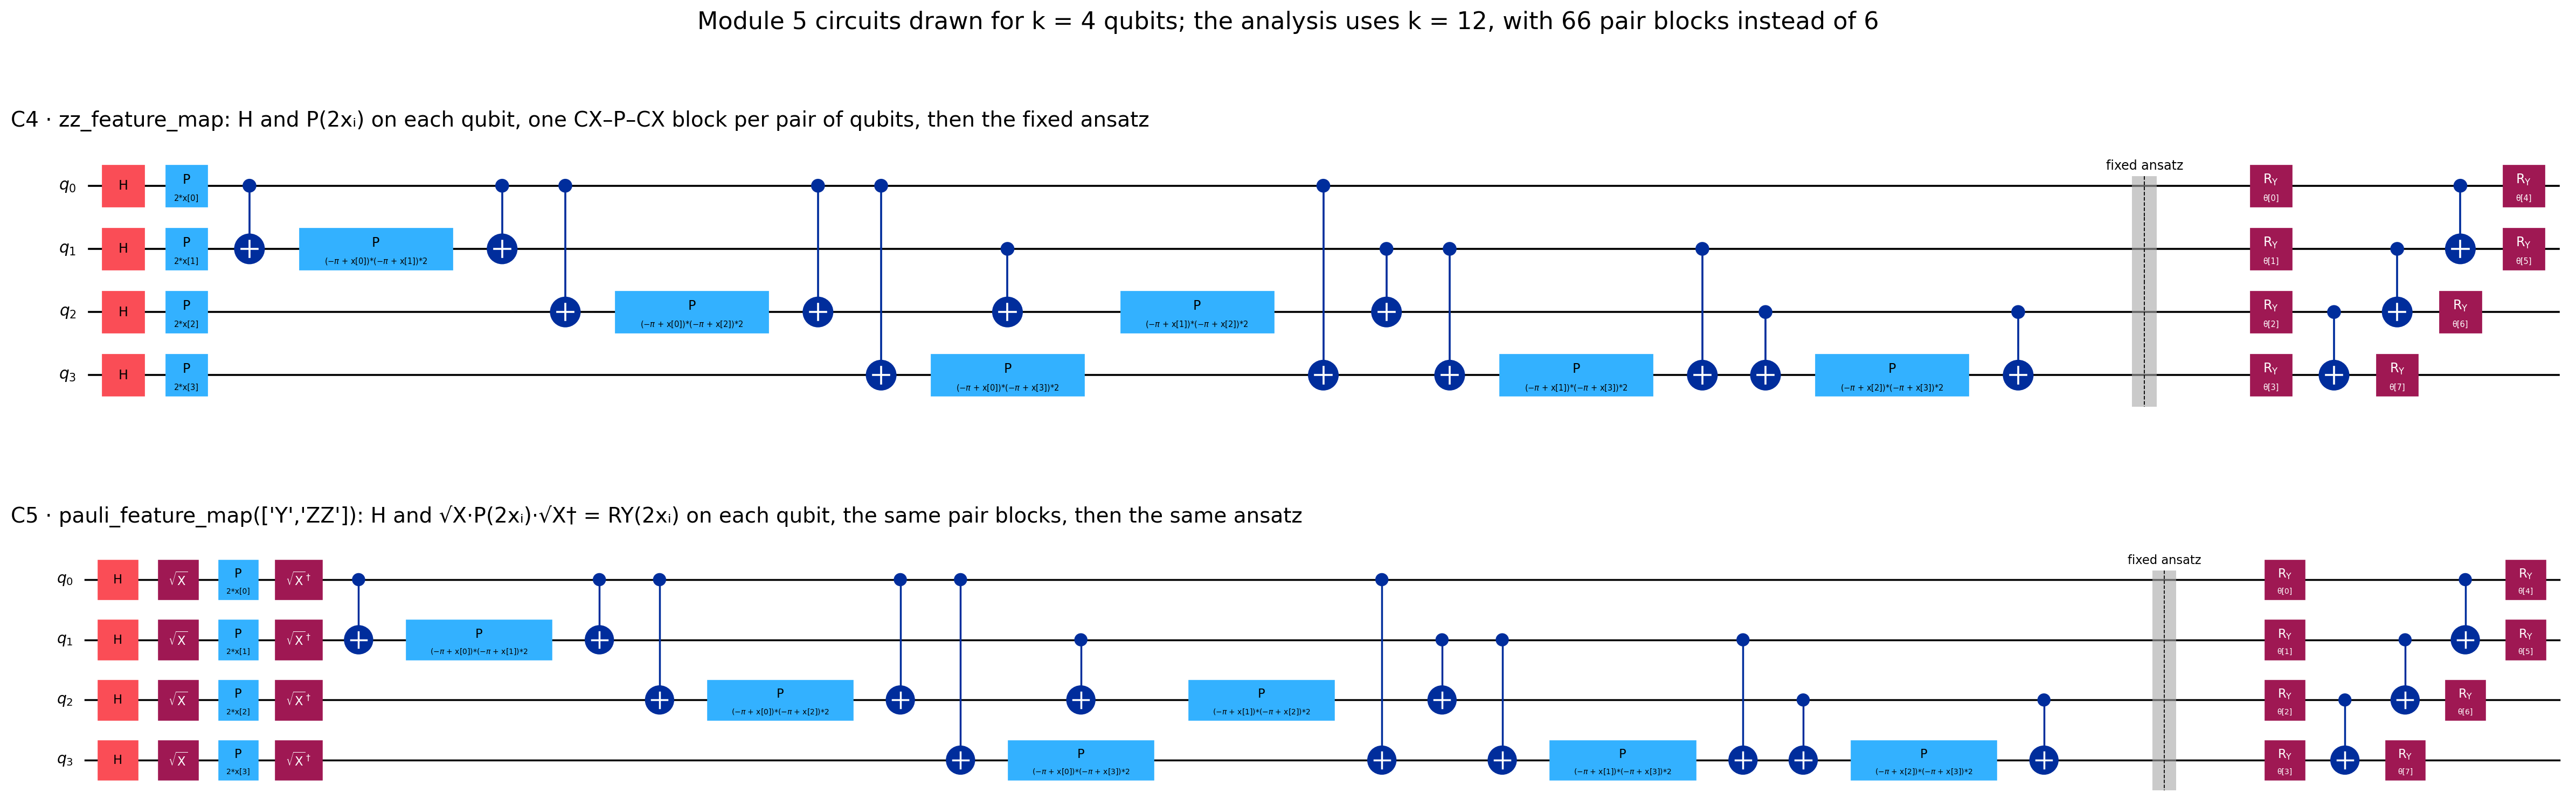
\includegraphics[width=\textwidth]{Figures/M5_circuit_k4.png}
\caption{Circuitos de C4 y C5 dibujados para $k=4$; el análisis usa $k=12$, con 66 bloques de pares en lugar de 6; la barrera separa el \textit{feature map} del \textit{ansatz} fijo.}
\label{fig:circuitos_k4}
\end{figure}
